\chapter{Proverbs 23}

\begin{figure}
  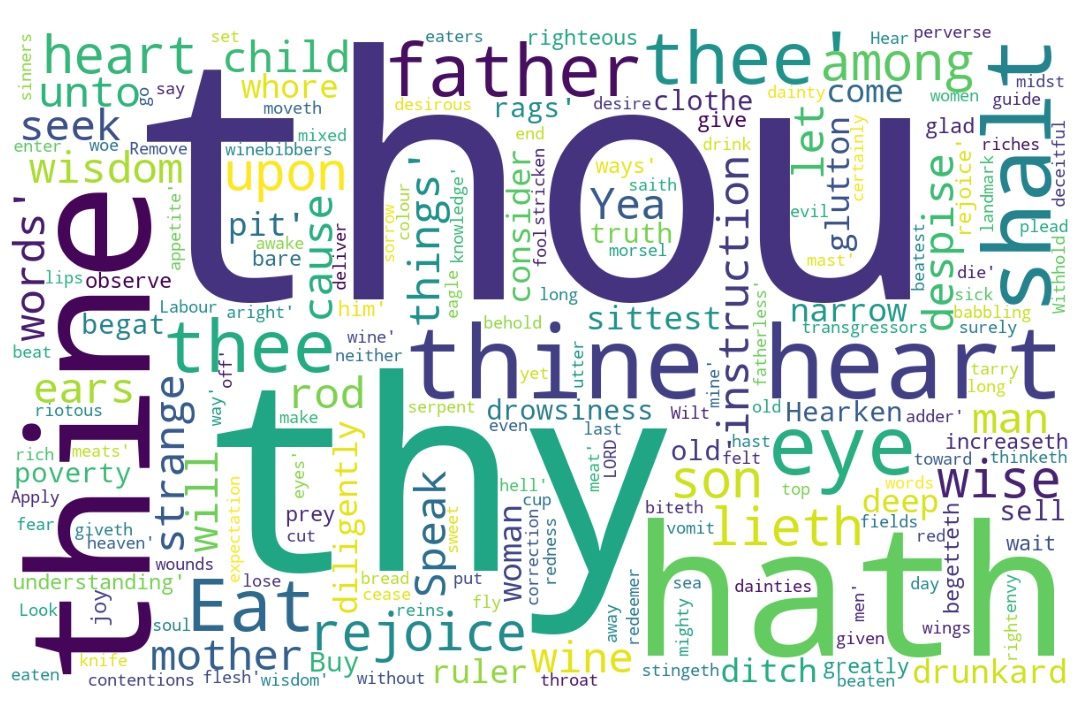
\includegraphics[width=\linewidth]{20OT-Proverbs/Proverb23-WordCloud.jpg}
  \caption{Proverb 23 Word Cloud}
  \label{fig:Proverb 23 Word Cloud}
\end{figure}


\marginpar{\scriptsize \centering  \fcolorbox{bone}{lime}{\textbf{STEPS TO RUIN}}\\ (Proverbs 23:1-35) \begin{compactenum}[I.][8]
    \item \textbf{Controlled by Flesh-eating (Appetite)} (\index[scripture]{Proverbs!Pro 23:01-03}Pro 23:1-3)
    \item \textbf{Compelled by Fantasy} (\index[scripture]{Proverbs!Pro 23:04}Pro 23:4)
    \item \textbf{Counseling Fools} (\index[scripture]{Proverbs!Pro 23:09}Pro 23:9)
    \item \textbf{Uncorrected by Fathers} (\index[scripture]{Proverbs!Pro 23:13}Pro 23:13)
    \item \textbf{Corrupted by Falsehoods} (\index[scripture]{Proverbs!Pro 23:16}Pro 23:16)
    \item \textbf{Consumed by ``Floosies'' (Whores)} (\index[scripture]{Proverbs!Pro 23:27}Pro 23:27)
    \item \textbf{Confused by Firewater} (\index[scripture]{Proverbs!Pro 23:29-35}Pro 23:29-35)
\end{compactenum}}


\marginpar{\scriptsize \centering \fcolorbox{bone}{yellow}{\textbf{A FOOL AND WISDOM}}\\ (Proverbs 23:1-35) \begin{compactenum}[I.][8]

    \item Wisdom is \textbf{Readily} available (\index[scripture]{Proverbs!Pro 23:09}Pro 23:9)
    \item Despises \textbf{Revelation} available (\index[scripture]{Proverbs!Pro 23:09}Pro 23:9)
    \item Becomes a Fool by \textbf{Rejection} (\index[scripture]{Proverbs!Pro 23:11}Pro 23:11)
    \item \textbf{Remains} a Fool by Rejecting (\index[scripture]{Proverbs!Pro 23:09}Pro 23:9)
    \item Associated with \textbf{Removing} Landmarks (\index[scripture]{Proverbs!Pro 23:10}Proverbs 23:10)
    \item At Odds with the \textbf{Redeemer}  (\index[scripture]{Proverbs!Pro 23:11}Pro 23:11)
    \item Slim Chance it Could be \textbf{Reversed}  (\index[scripture]{Proverbs!Pro 23:12}Pro 23:12)
\end{compactenum}}



% Choice, Child, Chastisement, Challenge [4]

\footnote{\textcolor[cmyk]{0.99998,1,0,0}{\hyperlink{TOC}{Return to end of Table of Contents.}}}\footnote{\href{https://www.audioverse.org/english/audiobibles/books/ENGKJV/O/Prov/1}{\textcolor[cmyk]{0.99998,1,0,0}{Proverbs Audio}}}\textcolor[cmyk]{0.99998,1,0,0}{When thou sittest to eat with a ruler,  \fcolorbox{bone}{lime}{consider diligently} what \emph{is} before thee:}
[2] \textcolor[cmyk]{0.99998,1,0,0}{And put a knife to thy throat, if thou \emph{be} a man given to appetite.}
[3] \textcolor[cmyk]{0.99998,1,0,0}{Be not desirous \fcolorbox{bone}{bone}{of} his dainties: for they \emph{are} deceitful meat.}
[4] \textcolor[cmyk]{0.99998,1,0,0}{ \fcolorbox{bone}{lime}{Labour}  \fcolorbox{bone}{lime}{not} to be rich: cease from thine own wisdom.}
[5] \textcolor[cmyk]{0.99998,1,0,0}{Wilt thou set thine eyes upon that which is not? for \emph{riches} certainly make themselves wings; they fly away as an eagle toward heaven.}
[6] \textcolor[cmyk]{0.99998,1,0,0}{Eat thou not the bread \fcolorbox{bone}{bone}{of} \emph{him} \emph{that} \emph{hath} an evil eye, neither desire thou his dainty meats:}
[7] \textcolor[cmyk]{0.99998,1,0,0}{For as he thinketh in his heart, so \emph{is} he: Eat and drink, saith he to thee; but his heart \emph{is} not with thee.}
[8] \textcolor[cmyk]{0.99998,1,0,0}{The morsel \emph{which} thou hast eaten shalt thou vomit up, and lose thy sweet words.}
[9] \textcolor[cmyk]{0.99998,1,0,0}{Speak not in the ears \fcolorbox{bone}{bone}{of} a  \fcolorbox{bone}{lime}{fool}: for he will despise the wisdom \fcolorbox{bone}{bone}{of} thy words.}
[10] \textcolor[cmyk]{0.99998,1,0,0}{Remove not the old landmark; and enter not into the fields \fcolorbox{bone}{bone}{of} the fatherless:}
[11] \textcolor[cmyk]{0.99998,1,0,0}{For their redeemer \emph{is} mighty; he shall plead their cause with thee.}
[12] \textcolor[cmyk]{0.99998,1,0,0}{Apply thine heart unto instruction, and thine ears to the words \fcolorbox{bone}{bone}{of} knowledge.}
[13] \textcolor[cmyk]{0.99998,1,0,0}{ \fcolorbox{bone}{lime}{Withhold not correction} from the child: for \emph{if} thou beatest him with the rod, he shall not die.}
[14] \textcolor[cmyk]{0.99998,1,0,0}{Thou shalt beat him with the rod, and shalt deliver his soul from hell.}
[15] \textcolor[cmyk]{0.99998,1,0,0}{My son, if thine heart be wise, my heart shall rejoice, even mine.}
[16] \textcolor[cmyk]{0.99998,1,0,0}{Yea, my reins shall rejoice, when thy lips speak  \fcolorbox{bone}{lime}{right things}.}
[17] \textcolor[cmyk]{0.99998,1,0,0}{Let not thine heart envy sinners: but \emph{be} \emph{thou} in the fear \fcolorbox{bone}{bone}{of} the LORD all the day long.}
[18] \textcolor[cmyk]{0.99998,1,0,0}{For surely there is an end; and thine expectation shall not be cut off.}
[19] \textcolor[cmyk]{0.99998,1,0,0}{Hear thou, my son, and be wise, and guide thine heart in the way.}
[20] \textcolor[cmyk]{0.99998,1,0,0}{Be not among winebibbers; among riotous eaters \fcolorbox{bone}{bone}{of} flesh:}
[21] \textcolor[cmyk]{0.99998,1,0,0}{For the drunkard and the glutton shall come to poverty: and drowsiness shall clothe \emph{a} \emph{man} with rags.}
[22] \textcolor[cmyk]{0.99998,1,0,0}{Hearken unto thy father that begat thee, and despise not thy mother when she is old.}
[23] \textcolor[cmyk]{0.99998,1,0,0}{Buy the truth, and sell \emph{it} not; \emph{also} wisdom, and instruction, and  \fcolorbox{bone}{MYGOLD}{understanding}.}
[24] \textcolor[cmyk]{0.99998,1,0,0}{The father \fcolorbox{bone}{bone}{of} the righteous shall greatly rejoice: and he that begetteth a wise \emph{child} shall have joy \fcolorbox{bone}{bone}{of} him.}
[25] \textcolor[cmyk]{0.99998,1,0,0}{Thy father and thy mother shall be glad, and she that bare thee shall rejoice.}
[26] \textcolor[cmyk]{0.99998,1,0,0}{My son, give me thine heart, and let thine eyes observe my ways.}
[27] \textcolor[cmyk]{0.99998,1,0,0}{For a whore \emph{is} a deep ditch; and a  \fcolorbox{bone}{lime}{strange woman} \emph{is} a narrow pit.}
[28] \textcolor[cmyk]{0.99998,1,0,0}{She also lieth in wait as \emph{for} a prey, and increaseth the  \fcolorbox{bone}{MYGOLD}{transgressors} among men.}
[29] \textcolor[cmyk]{0.99998,1,0,0}{Who hath woe? who hath sorrow? who hath contentions? who hath babbling? who hath wounds without cause? who hath redness \fcolorbox{bone}{bone}{of} eyes?}
[30] \textcolor[cmyk]{0.99998,1,0,0}{They that tarry long at the  \fcolorbox{bone}{lime}{wine}; they that go to seek mixed wine.}
[31] \textcolor[cmyk]{0.99998,1,0,0}{Look not thou upon the  \fcolorbox{bone}{lime}{wine} when it is red, when it giveth his colour in the cup, \emph{when} it moveth itself aright.}
[32] \textcolor[cmyk]{0.99998,1,0,0}{At the last it biteth like a serpent, and stingeth like an adder.}
[33] \textcolor[cmyk]{0.99998,1,0,0}{Thine eyes shall behold strange women, and thine heart shall utter perverse things.}
[34] \textcolor[cmyk]{0.99998,1,0,0}{Yea, thou shalt be as he that lieth down in the midst \fcolorbox{bone}{bone}{of} the sea, or as he that lieth upon the top \fcolorbox{bone}{bone}{of} a mast.}
[35] \textcolor[cmyk]{0.99998,1,0,0}{They have stricken me, \emph{shalt} \emph{thou} \emph{say,} \emph{and} I was not sick; they have beaten me, \emph{and} I felt \emph{it} not: when shall I awake? I will seek it yet again.}


